% THIS IS SIGPROC-SP.TEX - VERSION 3.1
% WORKS WITH V3.2SP OF ACM_PROC_ARTICLE-SP.CLS
% APRIL 2009
\documentclass{acm_proc_article-sp}
\usepackage[utf8]{inputenc}
\usepackage[english]{babel}
\usepackage{minted}
\usepackage{lineno}
\usepackage{hyperref}
\usepackage{enumitem}
\usepackage{amsmath}
\usepackage{tikz}
\usepackage{caption}
\usepackage{subcaption}
\usepackage{epigraph}
\usepackage{multirow}
\usepackage{tabularx}

%\usepackage{todonotes}
%\usepackage{marginnote} 
%\let\marginpar\marginnote

\usetikzlibrary{automata,arrows,positioning,calc,fit}
\linenumbers

\newcommand{\thesistitle}{Debugging Data-Flows in Reactive Programs}

\makeatletter
\newcommand\footnoteref[1]{\protected@xdef\@thefnmark{\ref{#1}}\@footnotemark}
\makeatother

\begin{document}

\title{\thesistitle}
%\subtitle{[Extended Abstract]}

\numberofauthors{3}
\author{
\alignauthor
Herman Banken\\
       \affaddr{Delft University of Technology, The Netherlands}\\
       \email{hermanb@ch.tudelft.nl}
\alignauthor
Georgios Gousios\\
       \affaddr{Delft University of Technology, The Netherlands}\\
       \email{g.gousios@tudelft.nl}
\alignauthor
Erik Meijer\\
       \affaddr{Delft University of Technology, The Netherlands}\\
       \email{h.j.m.meijer@tudelft.nl}
}

\date{\today} %10 Juli 2017}

\begin{minipage}[t][0.99\textheight]{0.99\textwidth}
%\begin{titlepage}
    \begin{center}
        \vspace*{1cm}
        
        \Huge
        \textbf{Visualizing Data-Flows \\in Reactive Programs}
        
        \large
		\vspace{0.5cm}
		by
        \vspace{0.5cm}
        
        \Large
        \textbf{Herman Banken}\\
		\normalsize
        born in Woerden, The Netherlands
        
        \vspace{1cm}
        \vfill

		to obtain the degree of Master of Science\\
		at the Delft University of Technology,\\
		to be defended publicly on Friday June 30, 2017 at 5:00 PM.
        
        \vspace{0.8cm}
                
		\begin{tabular}{l l l}
		Student number:     & \multicolumn{2}{l}{4078624} \\
		Project duration:   & \multicolumn{2}{l}{September 10, 2016 - June 29, 2017} \\
		Thesis committee:   & Prof. Dr. H.J.M. Meijer, 	& TU Delft \\
    						& Dr. G. Gousios,           & TU Delft \\
    						& Prof. Dr. A van Deursen,  & TU Delft \\
    						& Joost de Vries,           & Ordina
		\end{tabular}

        \vspace{0.8cm}

		An electronic version of this thesis is available at \url{http://repository.tudelft.nl}.

        
\includegraphics[width=5.76cm,height=2.72cm,natwidth=576,natheight=272]{images/logo.pdf}
    \end{center}
%\end{titlepage}
\end{minipage}

\maketitle
\begin{abstract}
Reactive Programming is way of programming designed to provide developers with the right abstractions for creating systems that use streams of data.
Adopting this new way of programming can be challenging, and without proper tooling even experienced developers sometimes struggle to comprehend complex reactive systems.
Traditional debug tools lack support for the abstractions provided, causing developers to fallback to the most rudimentary debug tool available: printf-debugging.

In this work, we design a visualization and debugging tool for Reactive Programming, that aids comprehension and debugging reactive systems, by visualizing the structure of the data flow and the data inside the flow.
We present RxFiddle, a platform for the visualization and the required instrumentation for RxJS in the ReactiveX-family of Reactive Programming libraries.
Evaluation based on an experiment shows that RxFiddle can outperform traditional debugging.

\end{abstract}

% A category with the (minimum) three required fields
%\category{H.4}{Information Systems Applications}{Miscellaneous}
%A category including the fourth, optional field follows...
%\category{D.2.8}{Software Engineering}{Metrics}[complexity measures, performance measures]

%\terms{Theory}

\keywords{reactive programming, debugging, visualization, program comprehension} % NOT required for Proceedings


% \documentclass{acm_proc_article-sp}
% \usepackage{graphicx}
% \usepackage{url}
% \usepackage{hyperref}
% \usepackage[top=1.25in, bottom=1.25in, left=1.25in, right=1.25in]{geometry}

% \hypersetup{ colorlinks=true, linkcolor=cyan, filecolor=cyan,
% urlcolor=cyan, citecolor=cyan, } \urlstyle{same}

% \def\sectionautorefname{section}

% \begin{document}

% \title{Visualizing Data-Flows in Reactive Programs}
% \author{ Herman Banken - 4078624
% \vspace{1cm} \\
% TU Delft, Department of Electrical Engineering, \\
% Mathematics and Computer Science }
% \date{\today}

% \vfill

% \begin{figure}[!bp]
%     \centering
%     \begin{minipage}[b]
%         {0.4\textwidth} 
\includegraphics[width=\textwidth,trim={0 12cm 0
%         10cm 0},clip]{images/tudelft.pdf}
%     \end{minipage}
%     \hfill
%     \begin{minipage}[b]
%         {0.4\textwidth} \includegraphics[width=\textwidth]{images/ordina.png}
%     \end{minipage}
% \end{figure}

% \maketitle

% \clearpage


\newcommand{\code}[1]{\texttt{#1}}
%\newenvironment{todo*}[1]{\textcolor{red}#1}{}
\newcommand{\todo}[1]{
\textcolor{red}{#1}
}
\newcommand{\todov}[1]{
{\color{red}
#1
}
}

% Stanford writing guide http://cs.stanford.edu/people/widom/paper-writing.html

\section{Introduction}
Software often needs to respond to external events and data flows. Consider software for example in interactive applications, for desktop, web and mobile phones, in graphics and in processing sensor data from phones or IoT-devices. We can use Reactive Programming (RP) to express the complex reactive behavior of these applications. RP offers declarative and concise syntax for composing streams of data. As a result programs are generally more comprehensible, when created using RP compared to an equal implementation using the Observer design pattern~\cite{johnson1995design, salvaneschi2014empirical}.

After receiving mostly academic interest for a long time in the form of FRP~\cite{elliott1997functional,elliott2009push,czaplicki2013asynchronous,maier2010deprecating} recent years brought RP to the developer community in the form of Flapjax~\cite{meyerovich2009flapjax}, Elm~\cite{czaplicki2012elm}, RxJS~\cite{meijer2010subject}, Angular (RxJS), React, Spring/Reactor and Akka Streams. Large companies like Netflix, Microsoft, Google and Facebook are betting on RP by working on these frameworks and libraries. As a result many developers are now starting to use RP.

%After researchers created research implementations of (Functional) Reactive Programming~\cite{elliott1997functional,cooper2006embedding,elliott2009push}  many production ready implementations are now available for commodity languages like JavaScript and Java.

%, compared to traditional programming approaches. As a result programs are generally more comprehensible, when created using RP compared to an equal implementation using the Observer design pattern~\cite{johnson1995design, salvaneschi2014empirical}.

While reactive programs might be more declarative and concise, RP does not work well with traditional interactive debuggers, shipped with most IDE's. RP borrows from Functional Programming (FP) for it's abstractions, its laziness and advocating the use of clean input/output (lambda) functions. All those features contribute to an execution flow that is mostly inside the RP implementation library, non-linear, resulting in not useful stack traces and frequently breakpoints don't help as relevant variables are not in scope. Furthermore, using a low level debugger makes it harder to see the high level relations and overview that the high-level RP abstraction provides.

\subsection{Motivation}
Understanding code is an important part of the daily life of a programmer. However, compared to programming in general, little is known about program comprehension and debugging practices for Reactive Programming. Existing knowledge about traditional imperative programs might not apply to RP. Many concepts of FP are borrowed by the RP libraries, about which Weck and Tichy say that ``higher-level abstractions like monads [...] can be a barrier for code comprehension"~\cite{weck2016visualizing}. Furthermore it is reiterated that there is a large gap between developers new to RP and experienced RP developers, at different occasions, including the recent Rx Contributor Days~\footnote{http://contributordays.com/contributor-days/rxjs}. To ``think in the reactive way'' requires comprehension of the core concepts that RP offers. As debugging is a fundamental part of comprehension, any improvements made to ease the debugging experience and capabilities in this area might improve how RP is comprehended.
The impact of any improvements on the developer community can be substantial, as recent reactive front-end frameworks like Angular and React grow in usage, and increasingly many developers are exposed to some form of RP. Doing something practically useful for this community is what lead us to create RxFiddle.

%In this paper we will first analyse
%
%Current debuggers are optimized for imperative programs, where statements are executed sequentially and control flow can be analyzed. 
%
%While the general behavior of programs becomes more comprehensible using RP, this does not necessarily hold in presence of complex operators, unintended behavior or faults. We define ‘debugging’ as examining the behavior of a program, and ‘debug-ability’ as a measure of debugging efficiency. To our knowledge no research exists which evaluates the debug-ability of reactive programming, and anecdotal evidence suggests existing tools are not sufficient[1].
%
%Traditionally faults are tracked down with the help of debugging: using breakpoints, logs and tests~\cite{zeller2009programs}). When debugging the execution of a sequential program the premises for control flow are known or computable using the current stack and heap, and the data flow can be followed by traversing down the stack trace. However, in RP events are triggered asynchronously, which resets the stack trace. The reset stack traces can not be traversed back to the previous event. Furthermore, this means previous stack frames containing data related to previous events are not accessible.
%
%This is especially challenging for more complex programs: while equal programs are easier to comprehend in RP style, more complex programs are also easily created, since RP also improves composability~\cite{maier2012deprecating}. These programs can be several degrees more complex in behavior than traditional applications.
%
%In summary, tracking down bugs becomes harder for two reasons:
%
%-   the search scope widens for larger applications
%
%-   existing tools are not sufficient for reactive programs.
%
%Specialized debuggers for reactive programming exist, although not as a result from academic research or with scientific validation. Examples are the Time Traveling Debugger (TTD) for Elm, a functional reactive programming (FRP) framework, and tools like RxVision and RxMarbles, which show that visualization is aids comprehension and debugging. Those tools fall short however: TTD is restricted to the Elm platform, RxVision is a mere proof of concept and restricted to the browser, and RxMarbles only visualizes a given set of operators, using fixed inputs.
%
%**Intended contributions.** In this thesis we will evaluate whether data or control flow graphs aid reactive program comprehension and debugging. Furthermore we present a tool which generates complete and interactive Marble Diagrams for full data flows, automatically, from sources and from running applications.

\subsection{Research Questions}
We formulate the following research questions to steer the research: 

\begin{description}
\item[RQ1] How do developers debug RP? \\
Before we design tools it is important to understand the problems arising in the the current state~\cite{singer2010examination}. Anecdotal evidence by a number of resources\footnote{http://contributordays.com/contributor-days/rxjs}\footnote{https://staltz.com/how-to-debug-rxjs-code.html}
suggests that the current state is non-optimal.

%	\begin{enumerate}
%		\item[RQ1.1] What strategies do developers use to comprehend RP?
%		\item[RQ1.2] What debug tools do developers use to comprehend \& debug RP?
%		\item[RQ1.3] {\color{orange}Do experienced developers debug RP faster?}
%	\end{enumerate}
%

\item[RQ2] How can we design a tool that helps developers debug RP? \\
Examining the limitations of traditional debuggers and the opportunities that RP programs offer in terms of structure and explicit dependencies between data flows, we design an RP debugger.

%	\begin{enumerate}
%		\item[RQ2.1] Can run-time behavior be extracted such that it is appropriate input to a visualizer?
%		\item[RQ2.2] Can Rx programs be represented as graphs?
%		\item[RQ2.3] Can Marble Diagrams effectively convey structures containing more than 1 operator?
%	\end{enumerate}

\item[RQ3] Can specialized debuggers speed up comprehension \& debugging? \\
To validate if specialized tooling can improve the experience we measure the speed and correctness of comprehension in both a controlled and in an online experiment.

%\end{enumerate}
\end{description}


\section{Background}
\label{background}
In this section we give an overview of related work 
and the context of this research.

\textbf{Debugging for Program Comprehension.}
Both debugging and comprehension are processes in the work of programmers.
Initially comprehension was seen as a distinct step programmers had to make
prior to being able to debug programs~\cite{katz1987debugging}, 
but this distinction is criticized by Gilmore saying we must view 
``debugging as a design activity''~\cite{gilmore1991models}, 
part of creating and comprehending programs. 
Maalej et al.~\cite{Maalej2014} interviewed professional developers 
and found that developers require runtime information to understand a program,
and that debugging is frequently used to gather this runtime information.
This supports our view that `debugging' is not only used for fault localisation,
but also for comprehension.
{\color{red}
\begin{enumerate}
 \item Gilmore, comprehension + debugging == linked
 \item Maalej: professionals, avoid deep comprehension, sharing knowlegde
 \item Maybe Zeller / Spinellis?
\end{enumerate}
}

\textbf{Dynamic Analysis.}
Although interactive debuggers are commonly used for comprehension 
of the runtime behavior of programs, more specialized tools exist: 
to study a programs execution is called `dynamic analysis' which has 
received substantial attention in the research community,
as surveyed by Cornellissen et al.~\cite{cornelissen2009systematic}.
They categorise on different facets being the 
\textit{activity} [goal of analysis],
\textit{target} [kind of inspected program or system],
\textit{method} [visualization, metrics, online, querying, etc.],
\textit{evaluation} [preliminary, case study, quantitative, etc.].
Most papers apply a \textit{post mortem} analysis, where first the program is run and then the trace data is analyzed to create a visualization.
Reis et al. mention the compromises
that have to be made to make an online analysis: 
reduced tracing is required to not slow down the 
system (known as the observer-effect), fast analysis 
and visualization is required to lower the cost of getting 
to the visualization, to not discourage the users.

Only X of the surveyed papers apply online analysis, rest post mortem.

{\color{red}
\begin{enumerate}
 \item Cornelissen, TU Delft, survey on Program Compr. through Dynamic Analysis
 		lists limitations: 
		   - incompleteness, only part of domain
			 - which scenarios to analyse
			 - scalability (wrt human cognitive load) 
		 	 - observer effect (multi-threaded, realtime) changes execution
\end{enumerate}
}

\textbf{Measuring Debugging.}
{\color{red}
\begin{enumerate}
	\item Minelli (know what you did last summer)
	\item Petrillo, "Towards Understanding..." e.g. Swarm debugging
  \item Moritz (watchdog 2.0)
\end{enumerate}
}

\textbf{Debugging for specific fields}
Most research into debugging focusses on procedural and 
imperative languages~\cite{cornelissen2009systematic}.
Other topics of interest are multi-threading and distributed systems.
Only few focus on other styles, like 
declarative programming~\cite{nilsson1998declarative}.
Debugging in reactive programming~\cite{
	salvaneschi2014empirical,salvaneschi2016debugging}.
	
{\color{red}
\begin{enumerate}
	\item Atlas (2014): rich graph representation, can be used to build call graphs, dataflow graphs, dependency graphs
	\item RP debugging (2016, Guido): REScala, data flow graph, breakpoints
	\item BIGDEBUG Spark debugging (2017): data flow graph, non-pausing simulated breakpoints, data provenance
\end{enumerate}
}

\textbf{Tracing \& Automated visualization for comprehension}
\begin{enumerate}\color{red}
 \item Lange 1995, Program Visualizer for C++
 \item story flow: visualize stories over time, comprehending relations, interactive visualization
 \item Weck \& Tichy, Visualizing Data-Flows in Functional Programs
 \item Srinivasan, ICPC16, "Case Studies of Optimized Sequence Diagram for Program Comprehension", Texas A\&M Univerity
 \item Misha Moroshko (Facebook) Rx visualization
\end{enumerate}

\subsection{Rx in a nutshell}
To understand how we create the visualization a minimal understanding of RP and the chosen implementation is required. Many RP implementations share a notion of a \textit{Observable}, which is a collection which abstracts over \textit{time}, in contrast to \textit{space} like standard collections.

Figure \ref{sample1} shows a very basic example of a in situ data flow in Rx. First an \textit{Observable} is created, here using the static \code{from} method, then dependent Observables are created using the \code{map} and \code{filter} methods on the Observable instance. Finally we \code{subscribe} to start the data flow and send the data in the flow to the console (eg. JavaScript's stdout).

\begin{figure}
\inputminted[tabsize=2]{javascript}{listings/sample1.js}	
\caption{Creation and transform of Observables}
\label{sample1}
\end{figure}

It is important to note that the Observable is lazy, it is the blueprint of a data flow. Only when you \code{subscribe} to an Observable the data flow is created by recursively subscribing up the stream. \textit{Observer}s are subscribed to each Observable until the source Observable is reached.
This is illustrated in figure \ref{dualgraphs}.
The origin of this design is the duality between Observables and \textit{Iterables}~\cite{meijer2010subject}, where Observers are dual to \textit{Iterators}.

Creating the Observable we will call the \textit{assembly} phase, the phase where the subscribe happens the \textit{subscription} phase and data flows in the \textit{runtime} phase. The three phases can be interleaved for different streams, for example when dealing with higher order Observables,  meaning one could use Observables as values inside the data flow. The Observables used as values have yet to start the second phase while the outer stream is in the runtime phase.

\begin{figure}
\begin{verbatim}
TODO nice figure with Graph & 2 lines (1 up, 1 down)
^ from(1, 2, 3)   			
^ .map(x => x * 2)       v
^ .filter(x => x > 2)    v
  .subscribe()           v
\end{verbatim}
\caption{Observable \& Observer dependencies}
\label{dualgraphs}
\end{figure}


\section{Research Design}
To answer our research questions we employ a mixed methods research approach as shown in Table~\ref{research-methods}.
First we interview professional developers and review available documentation (RQ1) to form a understanding about current debugging practices,
then we apply this understanding to design a debugger and implement it to test its feasibility (RQ2), 
finally we validate the debugger using an experiment (RQ3).

\begin{table*}[t]
\centering
\caption{Research Methods used in the study}
\label{research-methods}
\begin{tabular}{llll}
\hline
\textbf{}            & \textbf{Method} & \textbf{Type} & \textbf{Focus}                               \\ \hline
\multirow{2}{*}{RQ1} & Interview       & Qualitative   & What are current practices                   \\ \cline{2-4} 
                     & Literature      & Qualitative   & What is recommended                          \\ \hline
\multirow{2}{*}{RQ2} & Design          & Model         & What can a RP debugger show                  \\ \cline{2-4} 
                     & Implement       & Tool          & Collect the required meta information        \\ \hline
RQ3                  & Experiment      & Quantitative  & Quantification of effect on debug time       \\ \hline
\end{tabular}
\end{table*}

\iffalse
\todo{
qualitive data
quantitive
design, implemented, tested with real developers
buzz words: mixed methods, grounded theory
}
\fi

\section{RP Debugging practices}
\todo{alternative section titles: Evaluating motivation / collecting empirical evidence / case study}

To validate the need for better tools we must first understand what existing tools are used (RQ1).

\subsection{Literature and written work}
\todo{
\begin{itemize}
	\item clues in books: recent book (2016) on RP by Esposito and Ciceri~\cite{esposito2016reactive}, has chapter `Debugging' which solely consists of ways to print to the console and how to transform streams (by writing code) that are more easily printed.
	\item article by Stalz on how to debug\footnote{http://staltz.com/how-to-debug-rxjs-code.html}: iterates that there are 3 main ways: drawing the dependency graph, drawing marble diagrams, tracing to the console.
	\item Official documentation\footnote{\url{https://github.com/Reactive-Extensions/RxJS/blob/master/doc/gettingstarted/testing.md\#debugging-your-rx-application}}: use \code{do}-operator to add tracing to console.
\end{itemize}
}

\subsection{Interviews}
\todo{
Performed interviews in a professional setting. Questions asked include `how do you debug Rx', `how do you test Rx'. Answers gathered, using cards method, categorized to concepts.
}

%\todo{problem, solution, why choices made, motivate the choices}
%As discussed in Section ref{background}, much has been written about comprehension \& debugging programs in traditional settings, but little is known specific to RP. The fact that tooling like debuggers were designed for imperative languages suggests that the current debuggers might not be optimal for RP.
%
%Salvaneschi et al.~\cite{salvaneschi2016debugging} report that students use . This suggestion is strengthened by the experience of the first author in a professional setting that developers struggle with debugging Rx, sprinkling the code with \code{println}-statements in order to gain insight in the runtime behavior, instead of using standard features like breakpoints and stepping.

%The research is motivated by multiple factors. 
%
% Initially, the first author experienced existing debugging practices in a professional setting.  
%  anecdotal experience
%  
%  
%debugging practices RP unknown;
%
%Salvaneshi; professional experience; RQ1
%
%
%how to visualize RP?





\input{chapters/current}

\section{Debugger Design}
\label{section-design}
In this section we describe the design of a visualizer for the ReactiveX (Rx) family of RP libraries to answer RQ2. Given the findings of RQ1, the requirements for our visualizer are:
\begin{description}
\itemsep0em 
\item[REQ1] Provide overview of Observable flows
\item[REQ2] Provide detailed view inside flow
\end{description}

We propose a visualizer consisting of two parts: (1) a data flow graph and (2) a dynamic marble diagram. The data flow graph provides high-level overview, showing how different flows are created, combined and used, while the marble diagram offers a more in-depth look into a single selected data flow showing the contents (in terms of values and subscriptions) of the flows and can be used learn the behaviors and interplay of operators.

\subsection{Data Flow Graph}
\paragraph{Simplified graphs} When running an RP program, Observables are created that depend on other Observables (their \emph{source}) and Observers are created to send their values to a defined set of Observers (their \emph{destination}). Figure \ref{chaincreate} shows these relations in a graph. For the simplest of programs, the relations between the Observables ($O = {o_1, o_2, o_3}$) and those between Observers ($S = {s_1, s_2, s_3}$) share an equally shaped sub-graph after a reversal of the Observer-edges. To provide more overview, we process the graph to merge the two Observable and Observer sequences together, simplifying it in the process, as in Figure \ref{fiddlesimple}. Higher order relations are retained as shown in \ref{fiddlehigher}.

\begin{figure}[ht]
	\centering
	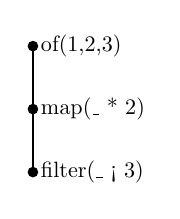
\begin{tikzpicture}[->,>=stealth',shorten >=1pt,auto,node
    distance=1.5cm,
                    semithick,scale=0.8, every node/.style={scale=0.8}]
    \tikzstyle{every state}=[] \filldraw (0,2) circle (2pt) node[right]
    {of(1,2,3)} -- (0,1) circle (2pt) node[right] {map(\_ * 2)} -- (0,0)
    circle (2pt) node[right] {filter(\_ < 3)};
\end{tikzpicture}

	\caption{Simplified graph of Figure \ref{chaincreate}}
	\label{fiddlesimple}
\end{figure}

\begin{figure}[ht]
	\centering
	
\begin{tikzpicture}[->,>=stealth',shorten >=1pt,auto,node
    distance=1.5cm,
                    semithick,scale=0.8, every node/.style={scale=0.8}]
    \tikzstyle{every state}=[] \filldraw (0,2) circle (2pt) node[right]
    {of(1,2,3)} -- (0,1) circle (2pt) node[right] {skip(1)} -- (0,0)
    circle (2pt) node[right] {flatMap(() => inner)};

    \filldraw (-1,1) circle (2pt) node[left] {of(`A', `B')} -- (0,0)
    circle (2pt) node[right] {};

    \filldraw (-0.7,1) circle (2pt) node[left] {} -- (0,0) circle (2pt)
    node[right] {};

\end{tikzpicture}

	\caption{Simplified graph of Figure \ref{chainhigher}}
	\label{fiddlehigher}
\end{figure}

\paragraph{Layout} Layout is used to add extra meaning to the graph. If multiple subscriptions on the same Observable are created, multiple flows are kept in the graph and they are bundled together in the resulting layout. This is designed to help developers find related flows. Also it is easy to see that for example an Observable is reused many times, hinting a possible performance improvement by sharing the computation (Rx has special \code{share}-operators to multicast). The layout is based on StoryFlow~\cite{liu2013storyflow}, which employs a hierarchical clustering before ordering the graph in a way to reduce crossings. Where StoryFlow clusters on physical character location we cluster flows per Observable. Furthermore, StoryFlow supports interactivity in various layout stages of which we use the algorithms for \emph{straightening} and \emph{dragging} to support selecting a specific flow, which is then highlighted, straightened and positioned at the right in order to match the marble diagram, shown for the current highlighted flow.

\paragraph{Color} Coloring the nodes can be used to identify the same Observable in multiple places in the graph, as Observables can be reused in different places of the stream.

\subsection{Dynamic Marble Diagrams}
In contrast to the original diagrams (Section \ref{marblediagram}) we use dynamic diagrams which update live when new events occur and are stacked to show the data in the complete flow. This allows the developer to trace a value back through the flow, a debug operation which is impossible using a classic debugger. Handcrafted marble diagrams can use custom shapes and colors to represent events, but for the generic debugger we use only three shapes: next-events are a green dot, errors a black cross, completes a vertical line, as shown in Figure~\ref{screenshot-mergeAll}. For our generic debugger it is unfeasible to automatically decide which properties (content, shape and color) to apply to events, as the amount of events and distinguishing features might be unbounded. Instead the event values are shown upon hovering.

\subsection{Architecture}
To support the visualization, we design a debugger architecture consisting of 2 components:

The \textbf{Host instrumentation} instruments the Rx library to emit useful execution events. Depending on the language and platform, specific instrumentation is required. Output of the instrumentation is a platform and language independent graph like Figure \ref{chainhigher}. By splitting the instrumentation, the debugger can be used for the complete ReactiveX family of libraries by only reimplementing the first component. The communication protocol for the instrumentation is shown in Table \ref{protocol}. 

The \textbf{Visualizer} takes the initial graph and simplifies it into a Data Flow Graph. Then it lays out the Data Flow Graph and provides the debuggers User Interface. By separating the visualizer, we can safely export generated graphs and visualize them post mortem for example for documentation purposes.

The components can run in their own environment. The instrumentation must run inside the host language, while the Visualizer can use a different language and platform.

\begin{figure*}
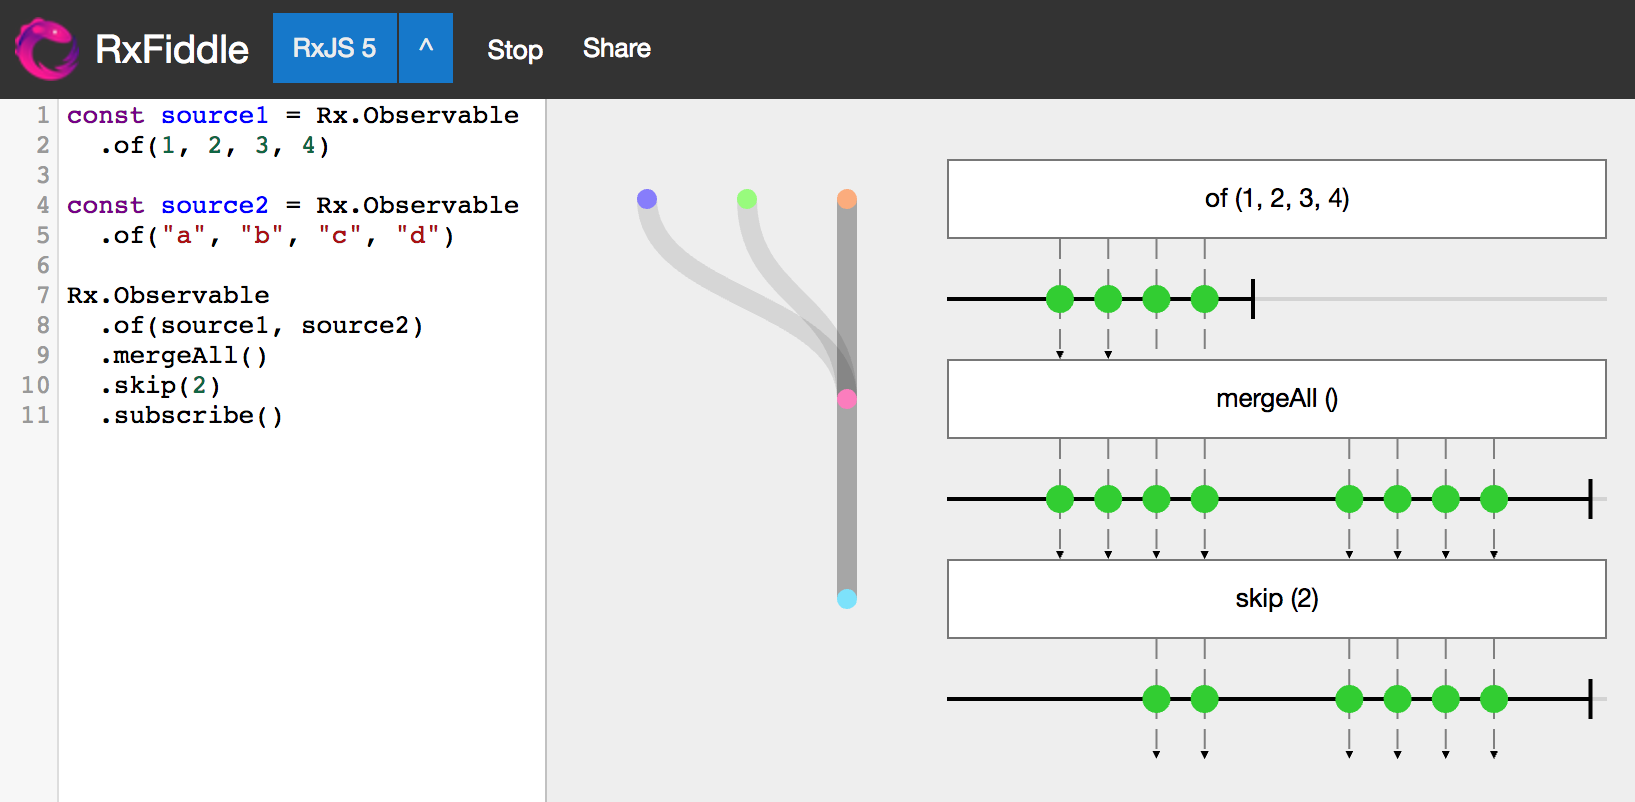
\includegraphics[width=\textwidth]{{images/screenshot.mergeAll.crop}.png}
\caption{Screenshot of \href{http://rxfiddle.net/\#type=editor&code=Y29uc3Qgc291cmNlMSA9IFJ4Lk9ic2VydmFibGUKICAub2YoMSwgMiwgMywgNCkKCmNvbnN0IHNvdXJjZTIgPSBSeC5PYnNlcnZhYmxlCiAgLm9mKCJhIiwgImIiLCAiYyIsICJkIikKClJ4Lk9ic2VydmFibGUKICAub2Yoc291cmNlMSwgc291cmNlMikKICAubWVyZ2VBbGwoKQogIC5za2lwKDIpCiAgLnN1YnNjcmliZSgp}{RxFiddle.net}}
\label{screenshot-mergeAll}
\end{figure*}

\begin{table*}[t]
\centering
\resizebox{\textwidth}{!}{%
\begin{tabular}{|l|l|}
\hline
addObservable(id, sourceIds)                   & Adds a Observable node, with zero or more source Observable's                                                                                                                      \\ \hline
addObserver(id, observableId, destinationId)   & \begin{tabular}[c]{@{}l@{}}Add a Observer, observableId denotes the Observable it subscribed to, \\ optional destinationId adds an edge to the destination Observer\end{tabular}   \\ \hline
addOuterObserver(observerId, outerDestination) & \begin{tabular}[c]{@{}l@{}}Create a special edge between an existing Observer and the higher order \\ destination Observer\end{tabular}                                            \\ \hline
addEvent(observerId, type, optionalValue)      & \begin{tabular}[c]{@{}l@{}}Add an event to the Observer denoted by observerId, of type (next, error, complete), \\ optionally with a value (for next / error events).\end{tabular} \\ \hline
addMeta(id, metadata)                          & Add meta data such as the method call which created an Observable.                                                                                                                 \\ \hline
\end{tabular}%
}
\caption{Instrumentation protocol}
\label{protocol}
\end{table*}

\subsection{Implementation}
To validate the design and to provide an implementation to the developer community we created \url{RxFiddle.net}. The RxFiddle project is a reference implementation of 
our reactive debugger design. Besides the visualizer, the website also contains a code editor for JavaScript code with sharing functionality, for developers to share snippets with their peers, as shown in Figure \ref{screenshot-mergeAll}. In this section we will explain different parts of the implementation. For RxFiddle, we initially focused on RxJS (JavaScript).

\paragraph{Instrumentation}
With JavaScript being a dynamic language, we use a combination of prototype patching and Proxies\footnote{\url{https://developer.mozilla.org/docs/Web/JavaScript/Reference/Global_Objects/Proxy}} to instrument the RxJS library: the Observable and Observer prototypes are patched to return Proxies wrapping the API method calls. The instrumentation passes every method entry and method exit to the Linking-step.

\paragraph{Linking}
Here, we distinguish between method calls from the different phases (Section \ref{nutshell}). From the assembly phase, we detect when Observables are used as target or arguments of a call or as return value, and create a graph node for each detected Observable. We add an edge between the call target \& call arguments and returned Observables, denoting the `source'-relation. Also, we tag the returned Observable with the call frame information (time, method name, arguments). In the subscription phase we detect calls to the \code{subscribe}-method: the destination Observers are passed as arguments, so we create the graph nodes and save the relation as an edge. In the runtime phase we detect `next', `error' and `complete' calls on Observers and add these as meta data to the Observer nodes.

\paragraph{Graph Loggers}
From the Linking-step the graph mutations are streamed to the environment of the visualizer, where the graph is rebuild. Depending on the host language a different protocol is used: RxFiddle's code editor executes the code in a Worker\footnote{\url{https://developer.mozilla.org/docs/Web/API/Worker}} and transmits events over the postMessage protocol, while RxFiddle for Node transmits over WebSockets. Being able to support multiple protocols increases the possible use cases, ranging from the code editor for small programs, to the Node plugin for server applications, to Chrome DevTool extensions\footnote{\url{https://developer.chrome.com/extensions/devtools}} for web applications.

\paragraph{Visualizer}
The visualizer receives the current state in the form of a graph from the Logger. It then uses the Observers in the graph to create the Data Flow Graph (DFG). 
To layout the DFG using StoryFlow~\cite{liu2013storyflow} we first rank the graph using depth first search, remove slack and reverse edges where necessary to create a directed acyclic graph. We then add dummy nodes to replaces long edges with edges spanning a single rank. Finally we order and align the nodes in the ranks assigning coordinates for the visualization. It is important that layout is fast, as it runs every time the DFG is changed. To render the Marble Diagrams the flow to and from the selected Observer is gathered by recursively traversing the graph in the direction of the edges, respectively the reversed direction.


\section{Evaluation}
For our RQ3, to validate our ideas about the debugger we designed an experiment to measure the (potential) speed up achieved with RxFiddle compared to the alternative of using the built-in Chrome Debugger.

\subsection{Experimental setup}

{\color{red}
\begin{verbatim}
controlled experiment at company
uncontrolled experiment online at RxFiddle.net
experiment includes:
- self assessment of programming skill
- self assessment of RP skill
- instruction video's
- non-question in question setting to familiarize with tooling
- warm-up question
- 3 questions involving different understanding/bugs:
  1. learning operator behavior (BMI sample)
  2. root cause analysis of crash
  3. analysis of timing bug, caused by wrong operator usage
\end{verbatim}
}

\subsection{Results}

{\color{red}
\begin{verbatim}
techniques to look into:
Wilcoxon
Cohen delta (normal) / Cliffs delta (non-normal)
check if normal distribution: Shapiro Wilks
\end{verbatim}
}


\subsection{Validity}
\textbf{Subjects.} The online experiment was open to anyone who wanted to participate. As a result a mixed group of developers took part, even those without Rx experience. The total amount of participants filling in the preliminary survey for the experiment was larger than the group finishing the experiment and some participants stopped during the tasks. We only consider results from fully completed tasks.

\textbf{Tasks.} The experiment consists of 2 small and 2 medium tasks, so the results of the experiment might not necessarily generalize to debugging RP in practice with larger systems. For larger tasks the effects of the debugger could be bigger and therefore be better measurable. Still we chose for these smaller tasks, for two reasons: in the limited time of the subjects they could answer only so many questions and designing larger tasks for the experiment would take many more iterations and time. With the limited amount of time available we still show that a significant speed-up can be achieved in some cases. We leave it for future work to extend the experiment to include larger systems.


\section{Discussion}


\section{Related Work}

\subsection{Debugging}
Debugging for general purpose languages revolves around 
attaching a debugger,
stepping through the code, 
attaching code or data breakpoints, 
navigating along different calls in the call stack and 
examining variables and results of expressions~\cite{Spinellis2017}.
However, existing research measuring how these different tasks are part of the developers work day found that 
while developers spend much time on comprehending code they do not spend much time inside the debugger~\cite{minelli2015know}.
Beller et al.~\cite{beller2017behavior} found that only 23\% of their subjects actively use the IDE's debugger,
with the most common action being adding breakpoints, followed by stepping through code.
The automated tooling of these studies did not measure different kinds of debugging other than using the IDE provided tools, 
however Beller's survey indicates that 71\% also uses printf statements for debugging.
No indication was given of any RP language and libraries used by the subjects in the study, 
but the observation that printf debugging is common matches our experience with debugging reactive programs.

% What comprises debugging?
% \item Maybe Zeller / Spinellis?

% \item Petrillo, ``Towards Understanding..." e.g. Swarm debugging
% \item Minelli (know what you did last summer)
% \item Moritz (watchdog 2.0)

\subsection{Debugging for Program Comprehension}
Both debugging and comprehension are processes in the work of programmers.
Initially comprehension was seen as a distinct step programmers had to make
prior to being able to debug programs~\cite{katz1987debugging}, 
but this distinction is criticized by Gilmore saying we must view 
``debugging as a design activity''~\cite{gilmore1991models}, 
part of creating and comprehending programs. 
Maalej et al.~\cite{Maalej2014} interviewed professional developers 
and found that developers require runtime information to understand a program,
and that debugging is frequently used to gather this runtime information.
This supports our view that `debugging' is not only used for fault localization,
but also for comprehension.

% \item Katz, distinct step
% \item Gilmore, comprehension + debugging == linked
% \item Maalej: professionals, avoid deep comprehension, sharing knowlegde

\textbf{Dynamic Analysis.}
Although interactive debuggers are commonly used for debugging 
of the runtime behavior of programs, more specialized tools already exist: 
the study of program execution is called `dynamic analysis' which has 
received substantial attention in the research community,
as surveyed by Cornellissen et al.~\cite{cornelissen2009systematic}.
They categorise on different facets being the 
\textit{activity} [goal of analysis],
\textit{target} [kind of inspected program or system],
\textit{method} [visualization, metrics, online, querying, etc.],
\textit{evaluation} [preliminary, case study, quantitative, etc.].
In most cases dynamic analysis involves a \textit{post mortem} analysis, 
where first the program is run and then the trace data is analyzed to create a visualization.
Reiss mentions the compromises that have to be made to make an online analysis~\cite{reiss2006visualizing}: 
reduced tracing is required to not slow down the system (known as the observer-effect), 
fast analysis is required to lower the cost of getting to the visualization, to not discourage the users.
In our design we found similar compromises relevant for RP debugging.

% \todo{
% \begin{enumerate}
%  \item Cornelissen, TU Delft, survey on Program Compr. through Dynamic Analysis
%  		lists limitations: 
% 		   - incompleteness, only part of domain
% 			 - which scenarios to analyse
% 			 - scalability (wrt human cognitive load) 
% 		 	 - observer effect (multi-threaded, realtime) changes execution
% \end{enumerate}
% }

\textbf{Specialized debuggers.}
Most research into debugging focusses on procedural and 
imperative languages~\cite{cornelissen2009systematic}.
Other topics of interest are multi-threading and distributed systems and 
only few focus on other styles, like declarative programming~\cite{nilsson1998declarative}.
Debugging specifically for Reactive Programming was only first mentioned and tried by Salvaneshi et al. for REScala~\cite{salvaneschi2014empirical,salvaneschi2016debugging}.

\todo{
\begin{enumerate}
	\item Atlas (2014): rich graph representation, can be used to build call graphs, dataflow graphs, dependency graphs
%	\item RP debugging (2016, Guido): REScala, data flow graph, breakpoints
%	\item BIGDEBUG Spark debugging (2017): data flow graph, non-pausing simulated breakpoints, data provenance
\end{enumerate}
}

\textbf{Tracing \& Automated visualization for comprehension}
\todo{
\begin{enumerate}
 \item Lange 1995, Program Visualizer for C++
 \item story flow: visualize stories over time, comprehending relations, interactive visualization
 \item Weck \& Tichy, Visualizing Data-Flows in Functional Programs
 \item Srinivasan, ICPC16, ``Case Studies of Optimized Sequence Diagram for Program Comprehension", Texas A\&M Univerity
%  \item Misha Moroshko (Facebook) Rx visualization
\end{enumerate}
}

\section{Conclusion}
In this paper, we presented RxFiddle, a debugger for reactive programs using RxJS. With RxFiddle developers can see the run-time data flow structure of their application and the events that go through these flows. We show that RxFiddle is an alternative for traditional debugging and in some cases outperforms traditional debugging in terms of time spend.

We plan to extend RxFiddle to other members of the Rx-family of languages. Furthermore we want to extend the debugger user interface to scale better and provide even more insight leveraging already captured meta data about timing of events.

%\include{scratchpad}

\bibliographystyle{unsrt}
\bibliographystyle{abbrv}
\bibliography{papers/references}

\appendix

\begin{figure*}[h]
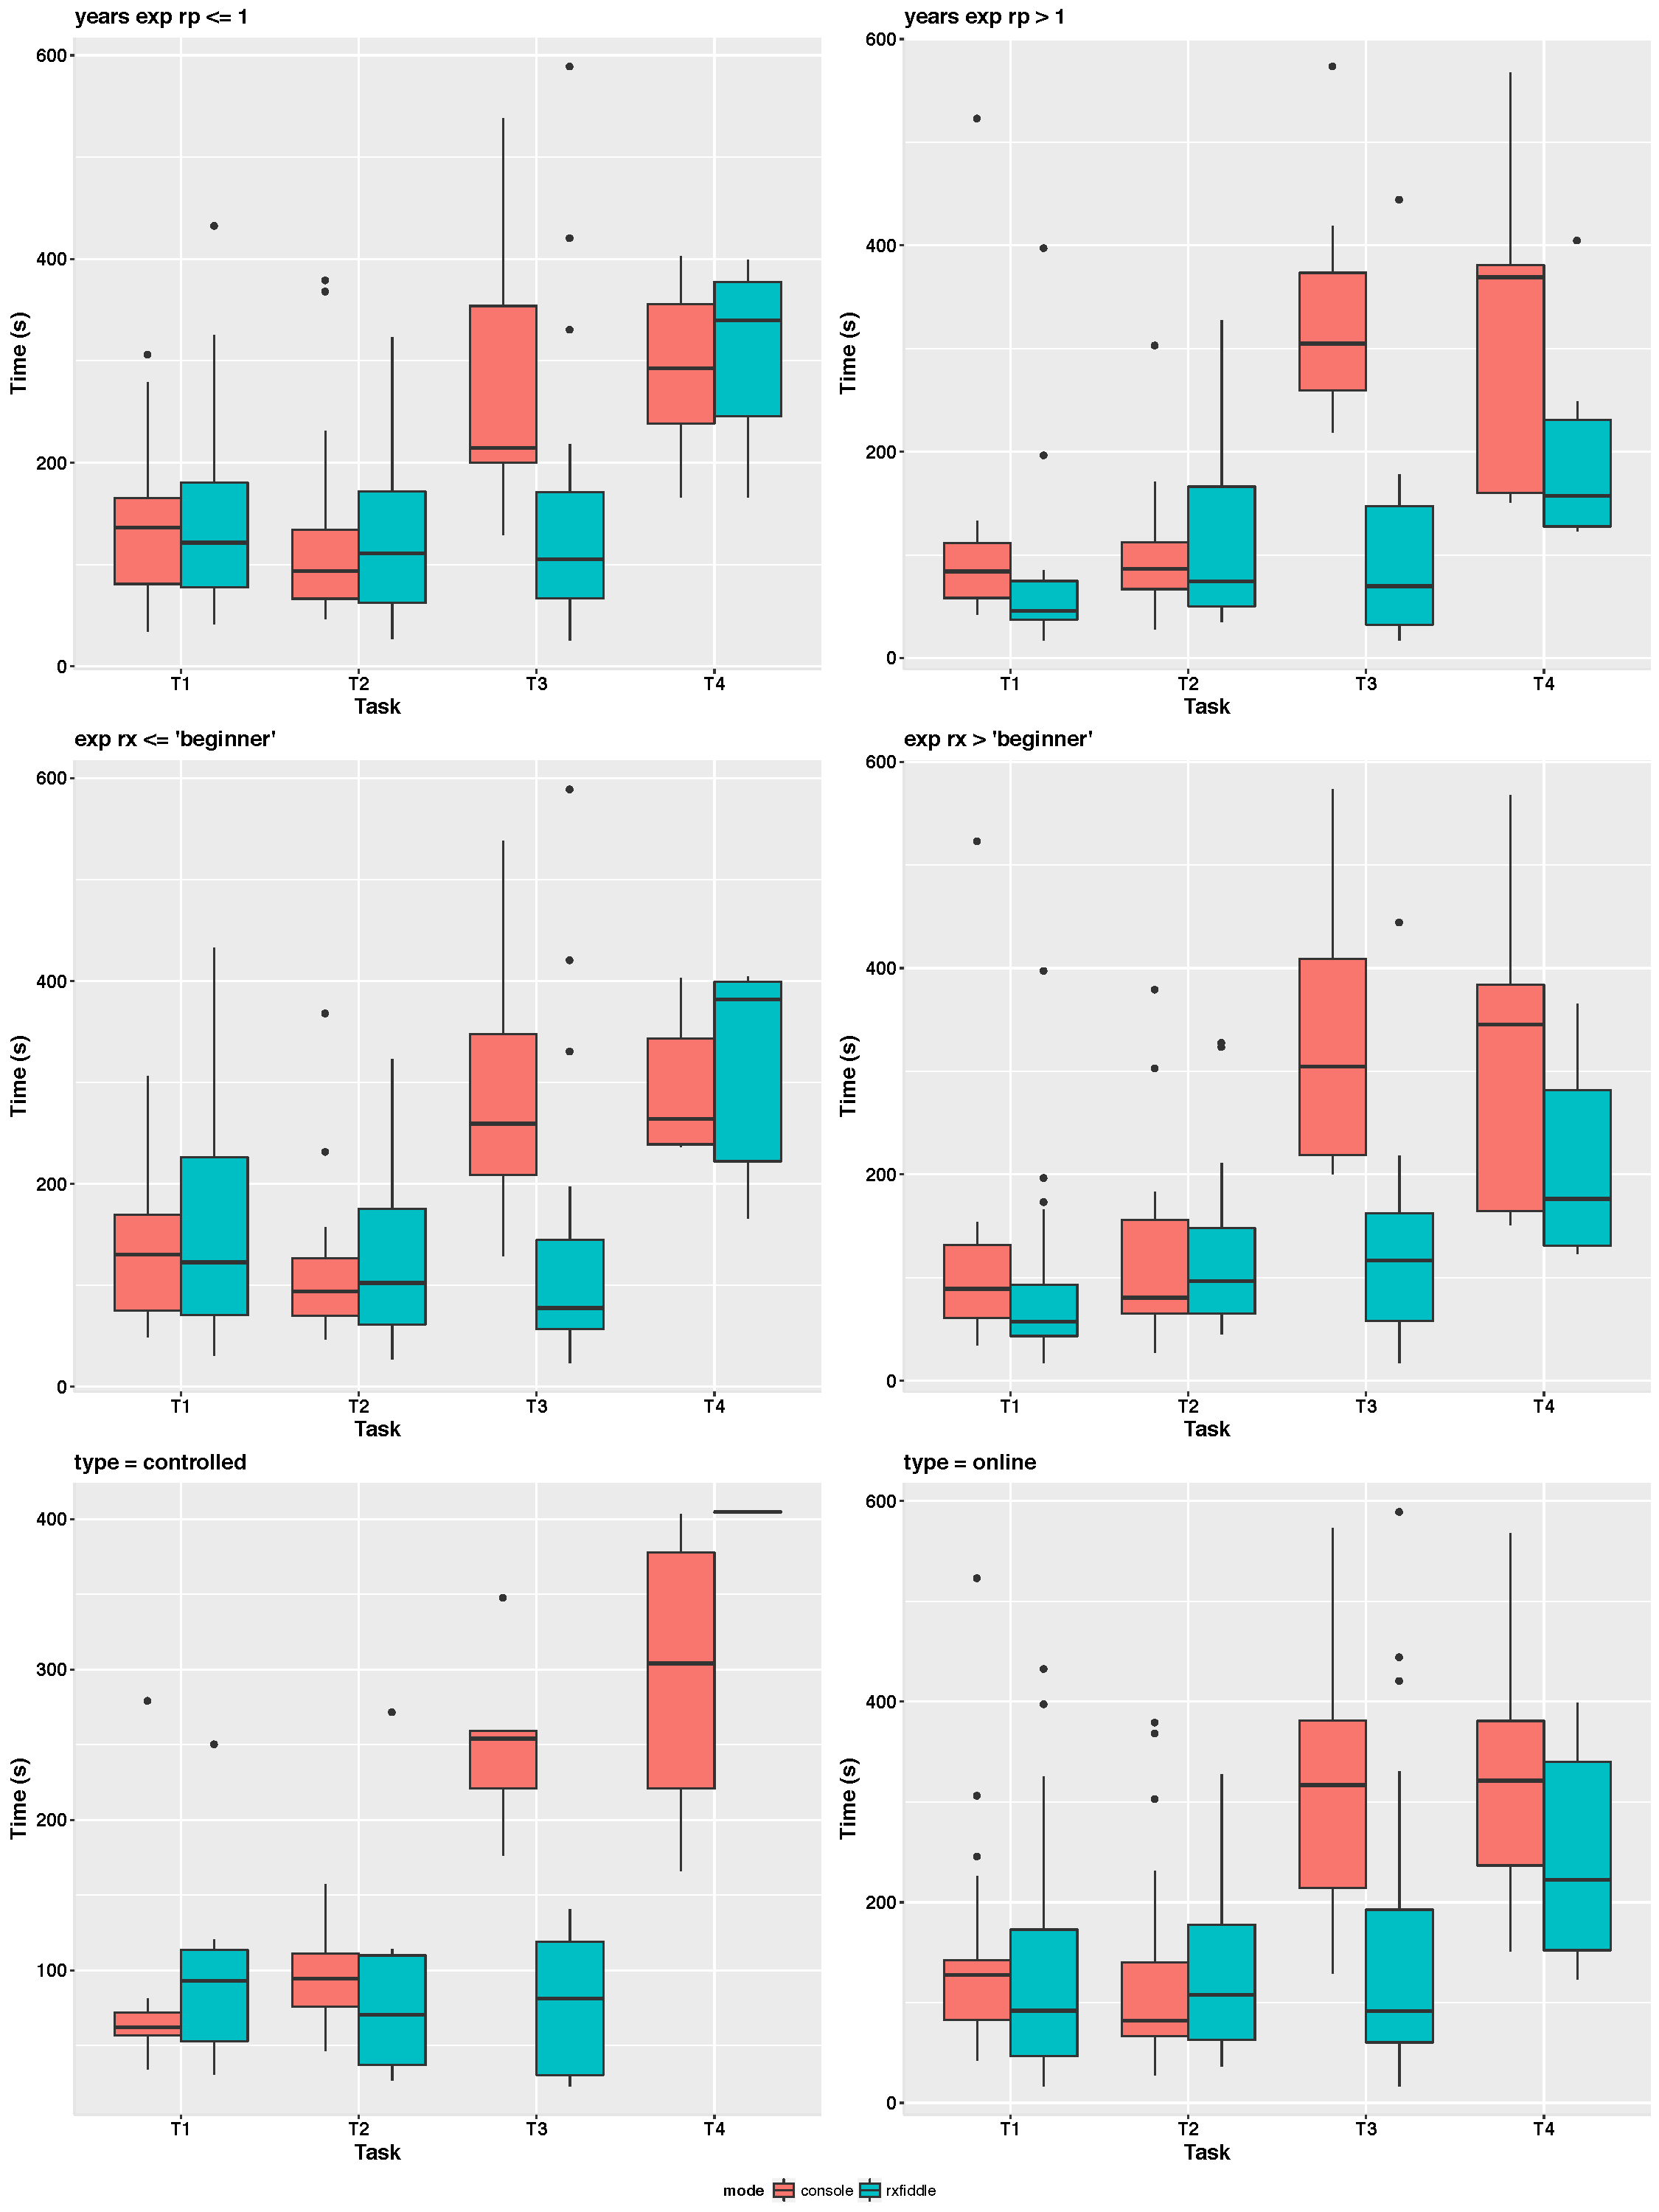
\includegraphics[width=\textwidth]{images/timePerTaskSplit.pdf}
\caption{Time until correct answer per task, split in various groups}
\label{fig-timePerTaskSplit}
\end{figure*}



\end{document}